\section{Where the intervention acts}
\label{sec:mechanism}

\begin{figure}[t]
  \centering
  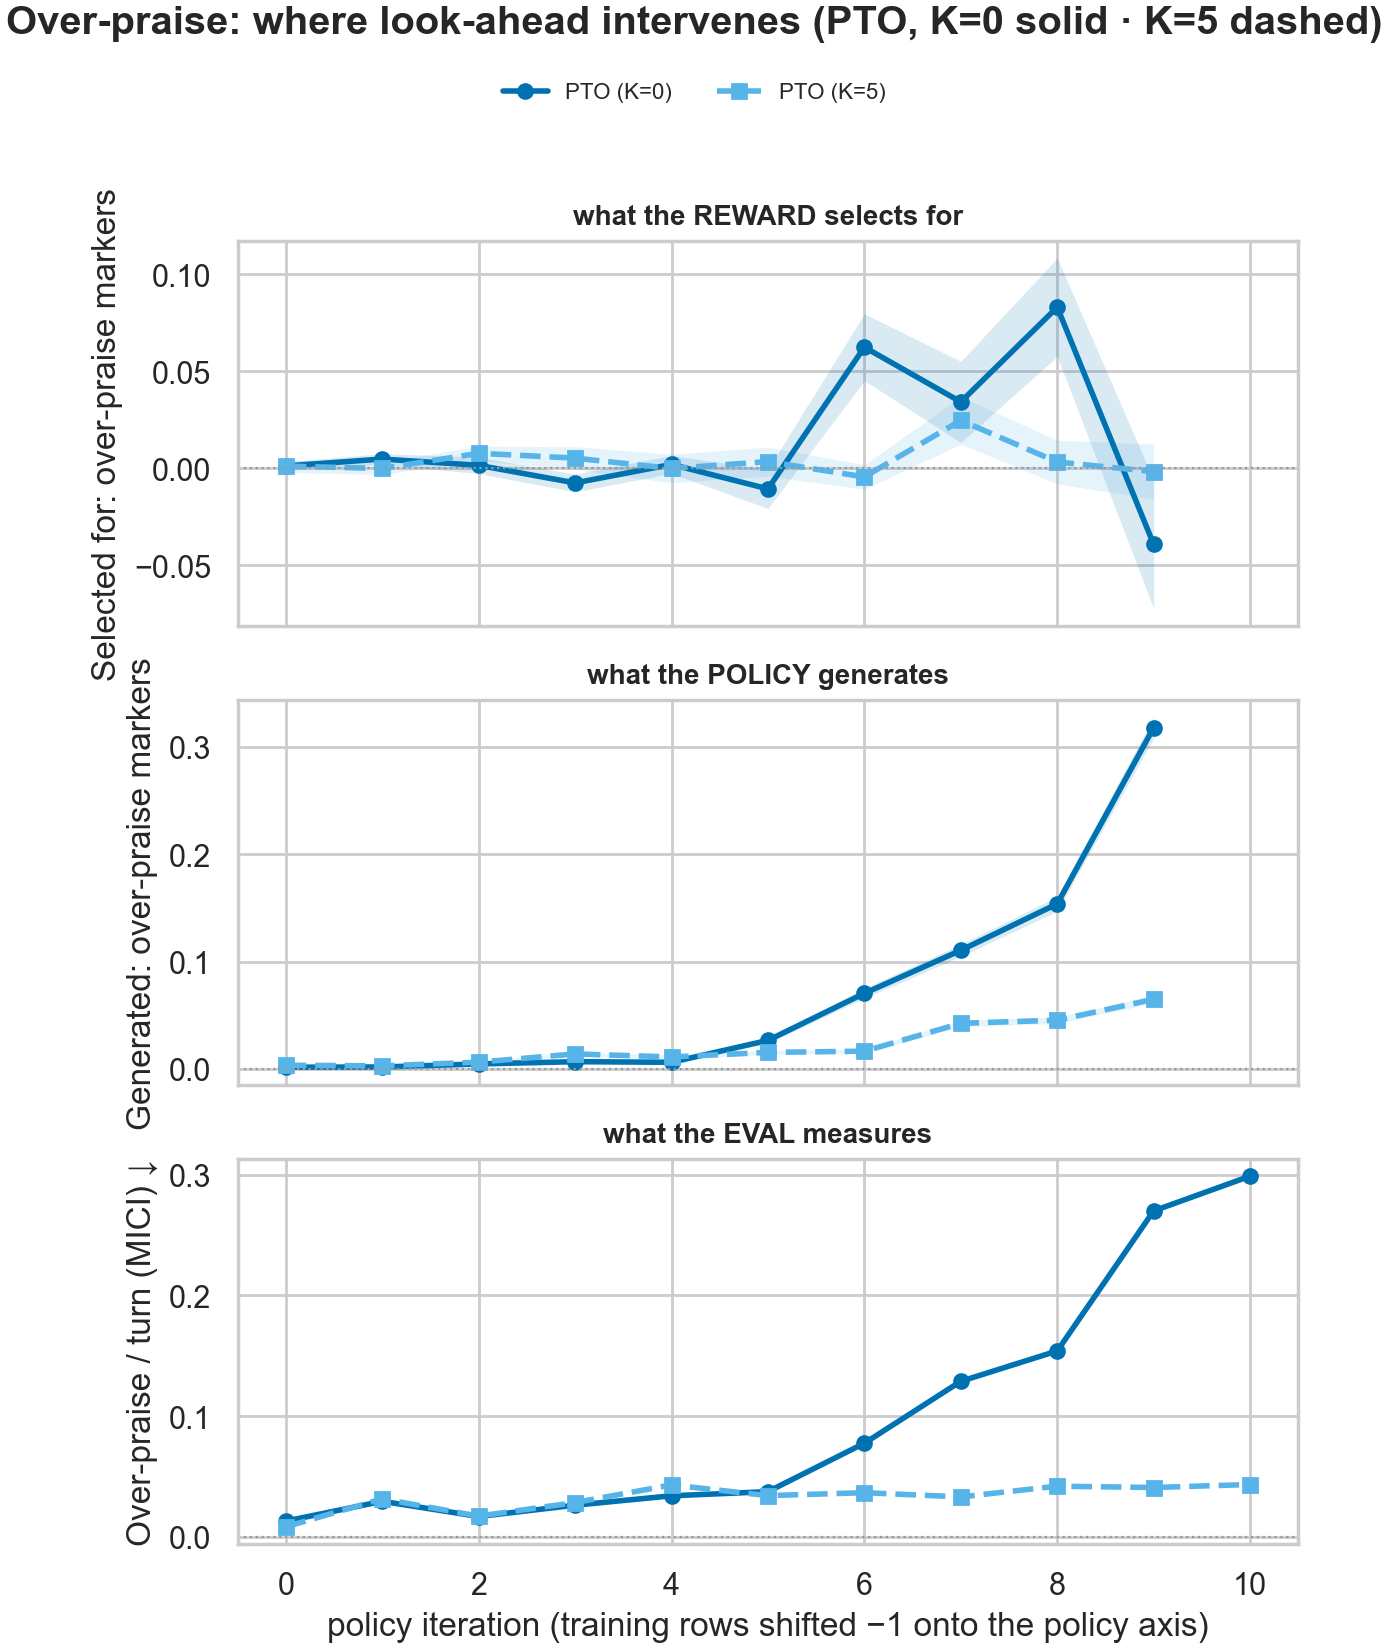
\includegraphics[width=\columnwidth]{figures/k_mechanism_overpraise_gpt-4o-mini.png}
  \caption{The over-praise channel at the three levels it must pass to become behaviour, both PTO
    arms. Top: what the reward selects for within a candidate group ($\pm 1$~SE). Middle: what the
    policy generates over \emph{all} candidates. Bottom: what the full-conversation evaluation
    measures. Training rows are shifted one iteration onto the policy axis, so all three describe
    the same policy. The \Kz{} selection weight lifts off around policy iteration~5, the pool
    follows, the evaluation follows; the \Kf{} arm is flat at every level.}
  \label{fig:mechanism}
\end{figure}

A behaviour reaches the policy through three gates: the reward has to prefer it within a candidate
group, the policy has to start producing it, and the evaluation has to observe it. An intervention
that only shows up at the third gate has not been explained.

Because every training group logs all its candidates with their oracle scores, we can measure the
first gate directly. For each iteration and arm we compute the within-group association between a
candidate's over-praise marker count and the weight the update gives it --- positive means the
update pushes the policy toward flattery, zero means it is indifferent. Figure~\ref{fig:mechanism}
stacks that against the candidate-pool mean and the evaluated rate.

The chain is consistent. Under \Kz{} the selection weight is indistinguishable from zero for five
iterations, rises to $+0.06$--$0.08$ at policy iterations 5--8, and the pool and the evaluation
follow with a lag. Under \Kf{} the selection weight never leaves zero (maximum $+0.025$), and
neither does anything downstream. Look-ahead is acting on the reward, not on the policy: with five
turns of continuation appended, a flattering turn stops being the higher-scoring member of its
group.

\paragraph{The pressure has to go somewhere.} This is also why the substitution is unsurprising in
hindsight. The optimiser's objective did not change and its capacity to find high-scoring turns did
not change; only the relative price of one route went up. What the trajectory-extended oracle still
rewards is a turn that makes the next five turns look productive, and on this client simulator
giving concrete advice does that at least as well as praising. Nothing in the intervention
penalises advice --- it penalises praise that does not compound.

\paragraph{Magnitudes.} Two numbers are worth holding together. The per-iteration selection
pressure on over-praise never exceeds $0.086$, an effect so small that a single update is
indistinguishable from indifference. The candidate pool's over-praise marker rate over the same
run moves from $0.002$ to $0.318$. A per-step bias too small to measure in isolation compounds,
through the on-policy loop, into the dominant feature of the policy's output --- which is why an
intervention has to be evaluated at the end of ten iterations of that loop and not at the end of
one. The $K{=}5$ arm's pool reaches only $0.065$ over the same ten iterations --- a factor of
$0.318 / 0.065 = 4.9$ below, having started from the same place. That factor is shrinking, not
holding: it was $7.5$ at iteration~8. The training-side gap is real and is narrowing.
